\chapter{Camera Calibration}\label{chap:camcalib}
\section{Overview}\label{sec:caliboverview}
Camera calibration of the data acquisition cameras is a fundamental first step in achieving accurately scaled reconstructions. It is a highly studied and in common setups a solved problem. While much of the research of the community has passed the calibration phase, it is still the fundamental first step in a number of vision based research topics. Accurate calibration models and properly undistorted images are a necessity for any kind of accurate depth measurements, 3D reconstructions, or robotic navigation through a physical space via imaging. Good calibration relies on good input image data and sometimes this can be difficult to obtain. Cameras without digital screens make it impossible to view images or video until connected to a computer. This can make it difficult to validate the calibration set up while gathering input. In the underwater domain, cameras that lack this feature make data validation much more tedious and time consuming as the cameras must be removed from the water and connected to an external machine. If the data is being recorded in the field without additional equipment, it may be impossible to view the images or footage until data collection is complete. This can be even more problematic for stereo calibration systems where it is important that both cameras record the required information. As such, identifying the subset of collected data that results in the best calibration model is an important step in the calibration process.  

With such factors as affordability, durability, and quality becoming commonplace for the camera market, the use of cameras in research has grown. One popular brand is GoPro which develops small, durable, high resolution action cameras. GoPro cameras can be used in a number of domains including above and below water and on a number of different applications such as building reconstruction or ocean floor mapping. While the popularity of these cameras has increased, they are susceptible to some of the challenges in collecting good calibration data. Most GoPro models lack a screen for viewing images and footage during and after capture making it hard to position the camera in the scene. Part of this problem has been fixed with the introduction of new Bluetooth and smart phone features, but wireless communication is severely limited in the underwater domain. In the case of this work, there was a need to accurately undistort footage obtained using GoPro's SuperView capture mode. This mode causes severe distortion along the edge of the frame which some calibration tools have trouble overcoming. 

\begin{figure}[t]
	\centering
	\fbox{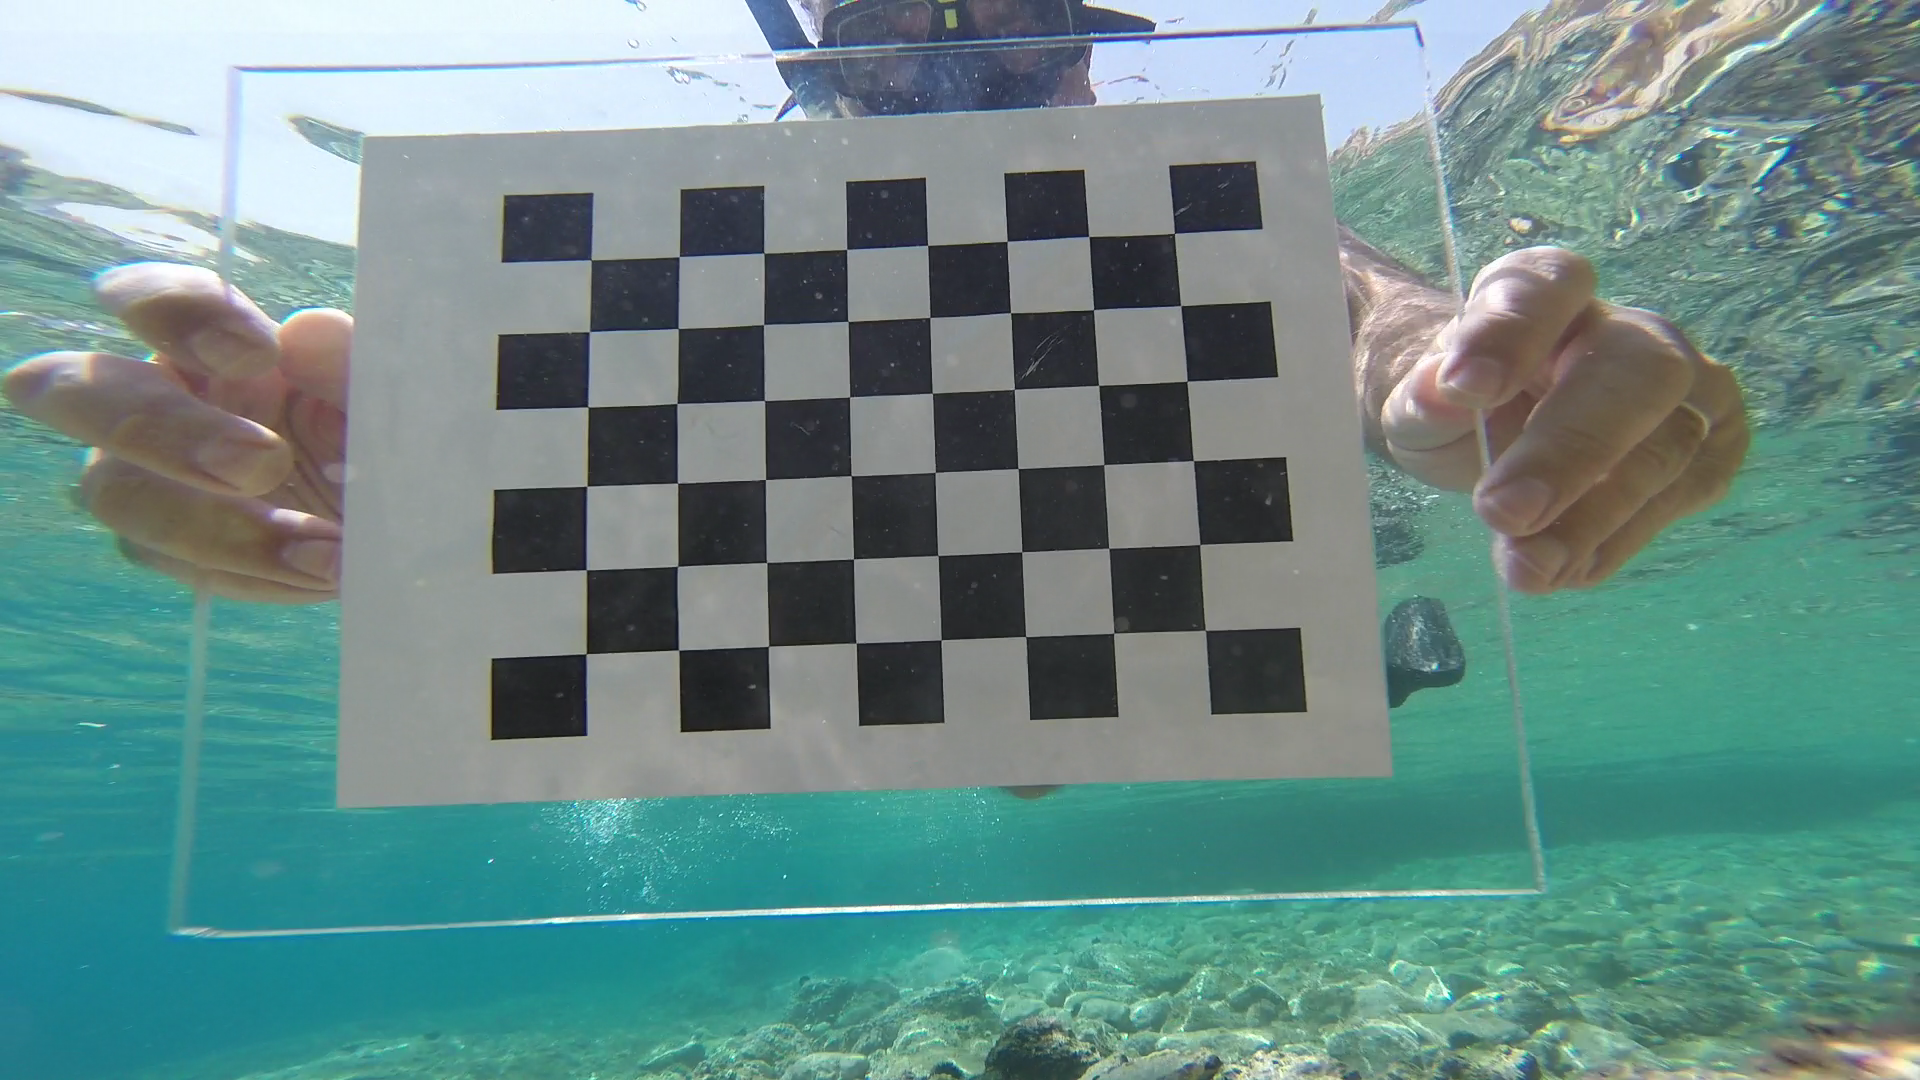
\includegraphics[width=0.75\textwidth]{./figures/right-0006.png}}
	\caption{An underwater image of a waterproof calibration checkerboard pattern used for camera calibration.}
	\label{fig:beauty}
\end{figure}

\section{Related Work}\label{sec:camrel}
Camera calibration is a well established method originating back to as early as the 1900s with lens research by Conrady~\cite{Conrady1919}. This developed into the Brown distortion model which forms the foundation for modern day camera calibration techniques~\cite{Brown1966,Brown1971,Brown1986}. One of the first openly available camera calibration tools was the Camera Calibration Toolbox for MATLAB. This tool, developed by Jean-Yves Bouguet, could calibrate a camera and return the intrinsic and extrinsic parameters. The toolbox was built on the foundation of work done by Tsai~\cite{Tsai1987} for introducing off the shelf technologies to camera calibration, Heikkila and Silven~\cite{Silven1997} for presenting an intrinsic calibration model, and most prominently Zhang for developing many of the techniques used in the toolbox~\cite{Zhang2000}. This work was later ported to OpenCV and used to develop the more powerful Computer Vision System Toolbox for MATLAB. These two tools are widely used in the field today. 

More complex calibration models have been developed to handle more complicated camera lenses taking into account different types of distortion. Specific methods to deal with extreme fisheye and barrel distortion have arose both in OpenCV and in independently released packages. Both the  Camera Calibration toolbox for MATLAB and OpenCV have a fisheye calibration model based on the work of Kannala and Brandt~\cite{Bradnt2006}. Scaramuzza have worked extensively with omnidirectional camera calibration and has developed his own MATLAB toolbox ~\cite{Scara2006_1,Scara2006_2,Scara2008_1,Scara2008_2}. Currently these are the state of the art readily available tools for rapid prototyping and used by the general public, each with its own advantages and disadvantages.

In recent years, there has been a push for the calibration of low cost and easily portable camera systems. With the development and continued advancement of products such as the GoPro, research has gone into the calibration and use of these cameras to solve imaging problems. Balletti et al. ~\cite{balletti2014calibration} explained many of the advantages of lightweight cameras including their ease to handle, capability of performing under extreme conditions, and providing high quality stills and video. They also explained methods for calibrating the cameras for reconstruction purposes. In the realm of underwater camera calibration, Schmidt and Rzhanov~\cite{schmidt2012measurement}, and Shortis~\cite{shortis2015calibration} compared the results and techniques for calibrating GoPro systems with the added distortion of water. These studies all fail to touch on the calibration of the GoPro camera when it is set to SuperView mode. 

\begin{figure}[t]
	\centering
	\fbox{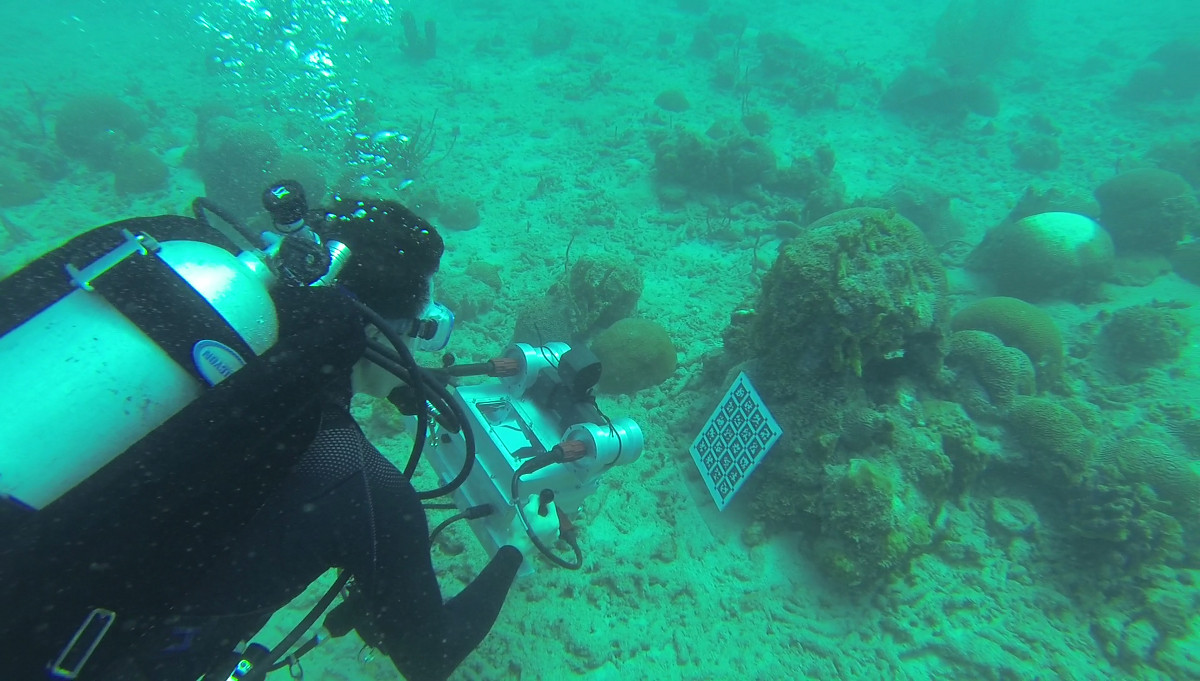
\includegraphics[width=0.9\textwidth]{figures/othersensors_red}}
	\caption{Diver calibrating an underwater rig consisting of stereo cameras and an IMU.}
	\label{fig:sensors}
\end{figure}

Calibration can be much more complicated and tedious if the camera is not the only sensor needing calibration. Many robotic systems take advantage of multiple proprioceptive and exteroceptive sensors in combination with visual input. A common proprioceptive sensor is the inertial measurement unit (IMU) which measures linear accelerations and angular velocities. Fig. \ref{fig:sensors} shows an example of the calibration process for a visual and interior sensor system. Significant efforts has been  in order to calibrate these systems as accurately as possible including the use of a Kalman Filter to determine the unknown coordinate transformations between sensors~\cite{4637877, doi:10.1177/0278364907079276, 2011_Kelly_Visual}. Because these calibrations rely heavily on the camera input, it is important that the camera calibration output is as accurate as possible so it will not skew the calibration of the other sensors. 



A system for assisting novice users to collect images for calibration through a Graphical User Interface is proposed by Richardson et al.~\cite{richardson2013iros}. 

Hu and Kantor~\cite{hu2016icra} presented a greedy approach for selecting images so that they are uniformly distributed over different camera poses. Such a method considers a budget that encodes the maximum processing time allowed. A quality metric could be considered to improve the performance.